%!TEX root = ../main.tex
\chapter{CALICE Calorimeter concepts}
\label{chap:CALICE_Det}

As explain in chapter \ref{chap:FutureColliders}, the ILC provides a clean environment for precision measurements. In many cases, the precision of the measurements is limited by the jet energy resolution. The jet energy resolution is itself limited by the energy resolution of the calorimeters (see section \ref{sec:PFA}). The jet energy resolution achieved by a traditional calorimetry is not sufficient for the ILC. A new approach called the Particle Flow is a promising solution to achieve an unprecedented jet energy resolution. The Particle Flow concept requires an excellent tracker and highly segmented electromagnetic and hadronic calorimeters. The \acrshort{calice} Collaboration is developing and testing highly granular electromagnetic and hadronic ca\-lo\-ri\-me\-ters concepts for a future linear collider optimized for Particle Flow.

In this chapter, after discussing the requirements for the calorimeters at the ILC in section \ref{sec:CaloRequirements}, various technology prototypes will be introduced in section \ref{sec:EMCal} and \ref{sec:HadCal} with a focus on the Analog Hadronic Calorimeter (AHCAL) in section \ref{sec:AHCAL}. The detection principle and readout electronics for the AHCAL are introduced in section \ref{sec:SiPM} and \ref{sec:SPIROC2B}.

\section{Requirements for the calorimeters in ILD}
\label{sec:CaloRequirements}

The objective for the ILC is to aim for a jet energy resolution of 3-4\%. Using traditional calorimetry, this is not achievable. Therefore, the particle flow concept was conceived to achieve this goal. With this approach, around 10\% of the jet energy is measured in the HCAL with a poor resolution. The particle flow concept imposes requirements on the calorimeters to achieve this goal.

One of the main requirements is the granularity of the calorimeters in order to be able to distinguish energy deposits from different particles. High granularity introduces new challenges that needs to be overcome such as the number of readout channels. Each channel needs its dedicated power and signal data lines for configuration and sensor readout. In traditional calorimeters, the number of channels is generally small and this approach can be done but in the case of highly granular calorimeters containing millions of channels, it is not feasible. One possibility to solve this is by integrating the front-end electronics on the active layers therefore, reducing the amount of power and data lines going in and out of the detector.

Additionally, other constraints are imposed to the calorimeters by the ILD detector. Theses constraints include mechanics, power consumption and power dissipation. In order to avoid dead material zones, there is no active cooling considered in ILD between calorimeter absorbers. Thus, this imposes a constrain on the maximum power dissipation by the front-end electronics on the active layers. To reduce the power consumption and dissipation, the front-end has to take advantage of the ILC beam structure. As shown in section \ref{sec:ILC}, ILC bunches are separated by 200 ms with each bunches being around 1 ms long. This leaves 199 ms where there is no collisions therefore, parts of the front-end electronics that are not needed can be switched off to reduce the power consumption and dissipation. This scheme is known as \textit{power-pulsing}.

\section{The CALICE Collaboration}

The \acrshort{calice} Collaboration is composed of scientists and engineers from all around the world who are developing and testing highly granular electromagnetic and hadronic ca\-lo\-ri\-me\-ters. These detector concepts are optimized toward a linear collider environment such as the International Linear Collider (ILC) \cite{ILC_TDR_Vol1} or Compact Linear Collider (\acrshort{clic}) \cite{CLIC_CDR} but a collaboration with the Large Hadron Collider community for the High-Lumi upgrade (HL-LHC) is ongoing \cite{1748-0221-12-01-C01042}.

The CALICE calorimeters are high granularity calorimeters optimized for the use of particle flow algorithms, see section \ref{sec:PFA}, providing a very detailed image of physics events and a high spatial resolution to separate nearby showers.

All the calorimeters developed within the collaboration are sampling calorimeters. Several \textit{physics prototypes} were build in the past and tested in testbeam campaigns at DESY, CERN and FNAL \cite{1748-0221-3-08-P08001, 1748-0221-5-05-P05004, 1707.07126v2, 1748-0221-10-10-P10039, 1748-0221-3-05-P05001} to demonstrate the principle of particle flow. Three prototypes of 1 m$^3$ were conceived using different active material and absorbers as well different readout schemes.

Nowadays, the CALICE Collaboration focuses on in the integration and scalability into a full linear collider detector by designing several new \textit{technological calorimeter prototypes}.

In the following sections, different electromagnetic and hadronic calorimeter concepts will be introduced before focusing on the main topic for this thesis, the CALICE AHCAL.

\section{Electromagnetic Calorimeters}
\label{sec:EMCal}

The CALICE collaboration is developing two different electromagnetic calorimeters con\-cepts. The goal of the previous prototypes was to prove the performance of such ca\-lo\-ri\-me\-ters for detailed measurements of EM showers. Now engineering prototypes are designed in order to improve the calorimeter design, the integration of the front-end electronics and the readout scheme. In the next subsections, the silicon-based SiECAL and the scintillator-based ScECAL calorimeters using both tungsten as absorber material will be described.

\subsection{Silicon-Tungsten ECAL}

The Silicon-Tungsten ECAL (SiECAL) physics prototype \cite{1748-0221-3-08-P08001} consists of 30 active and absorber layers. The depth of the calorimeter was 24 X$_0$ achieved by 10 layers of 0.4 X$_0$ (1.4 mm), followed by 10 layers of 0.8 X$_0$ (2.8 mm) and 10 more layers of 1.2 X$_0$ (4.2 mm) thick tungsten absorber plates. Tungsten has a small Moli\`ere radius of $\sim$9 mm and radiation length $\sim$3.5 mm, which allows for a compact design as well as compact electromagnetic showers in order to reduce the probability of overlapping showers.

The sensitive layer is made of high-resistivity silicon wafers 525 \si{\micro\meter} thick. These are divided into 6$\times$6 cm$^2$ sensors, segmented into a matrix of 1$\times$1 cm$^2$ PIN diodes operated in reversed bias. The total active area is 18$\times$18 cm$^2$ per layer. The SiECAL features 9720 channels. Silicon is a technology that is used for vertex and tracking detectors and can be segmented easily thus making it suitable for highly granular calorimeters. However, in the case of a calorimeter, the area to cover is large which makes this technology expensive in large-scale experiments.

No front-end electronic was integrated into the layers but placed off-detector using analog lines. A schematic of the prototype is shown in figure \ref{fig:SiWECALPhysics}. The performance of such calorimeter was tested in various beams at DESY and CERN. An energy resolution of $\frac{16.53\%}{\sqrt{E}}$ stochastic term and $1.07\%$ constant term was achieved \cite{ADLOFF2009372}.

\begin{figure}[htbp!]
  \centering
  \begin{subfigure}[t]{0.49\textwidth}
    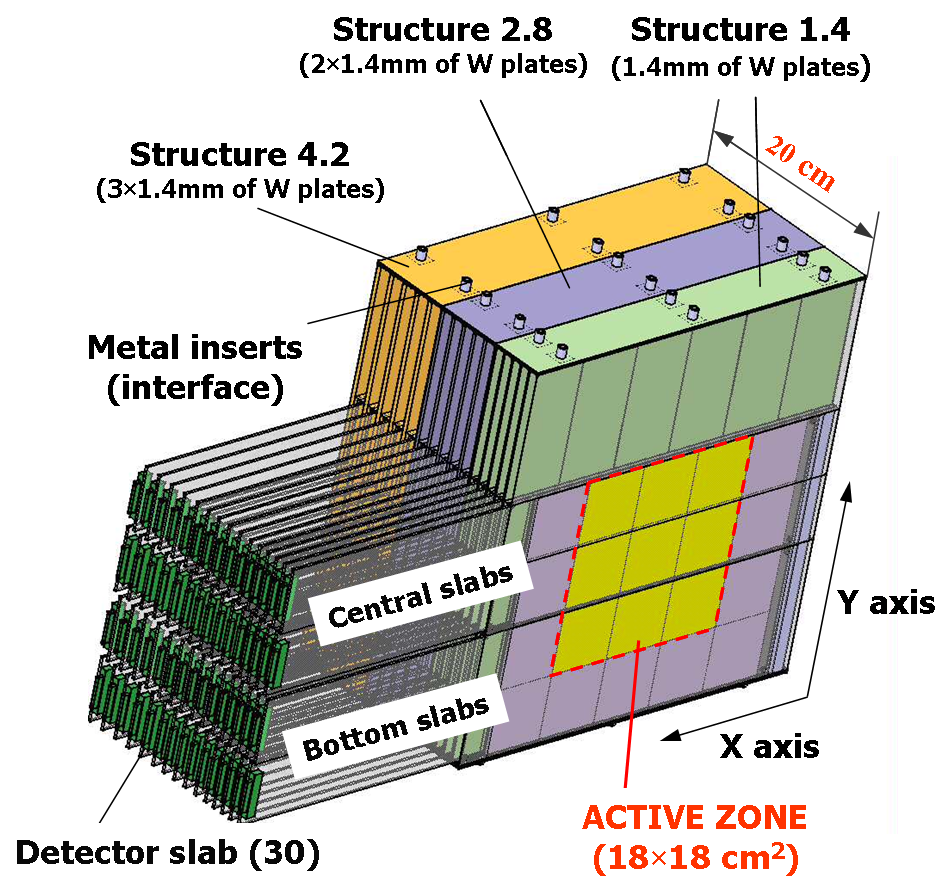
\includegraphics[width=1.\linewidth]{chap3/fig/3DProtoH.png}
    \caption{} \label{fig:SiWECALPhysics}
  \end{subfigure}
  \hfill
  \begin{subfigure}[t]{0.49\textwidth}
    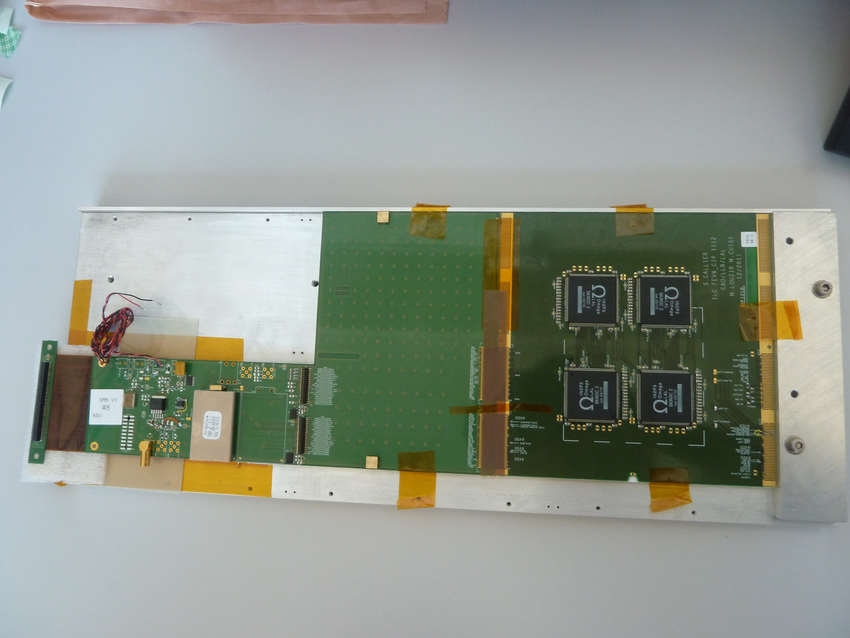
\includegraphics[width=1.\linewidth]{chap3/fig/SiW-ECAL_Techno.png}
    \caption{} \label{fig:SiWECALTechno}
  \end{subfigure}
  \caption{\subref{fig:SiWECALPhysics}) The schematics of the SiW-ECAL physics prototype. \subref{fig:SiWECALTechno}) Picture of a layer of the SiW-ECAL technological prototype.}
\end{figure}

After the validation of the calorimeter concept, a technological SiECAL prototype is being developed focusing on the integration into a full linear collider detector. To do this, modules close to the ILD design are being developed taking into account mass-production requirements and low-power front-end electronics are integrated into the detector volume. The silicon wafers are larger and divided into 9$\times$9 cm$^2$ sensors. The PIN diode matrix is reduced to 5$\times$5 mm$^2$ pads to improve the pattern recognition of the calorimeter. New designs of the sensor are also made to minimize dead area at the sensor edge and cross-talk effects.

The front-end is equipped with an \acrshort{asic}, the \acrshort{skiroc2} chip \cite{1748-0221-6-12-C12040}. It has 64 channels with adjustable gain charge pre-amplifier, a 12-bit \acrshort{adc} and digital logic. It allows for auto-triggering with an adjustable threshold and it can record the hit time performed on a 12-bit \acrshort{tdc} ramp. The SKIROC2 ASIC is designed to match the ILC beam structure (see chapter \ref{chap:FutureColliders}) and thus allows for a power-pulsed mode where electronics are switched off between ILC bunches. This allows a very low power dissipation in the order of 25 \si{\micro\watt} per channel. A picture of a layer of the technological prototype can be seen in figure \ref{fig:SiWECALTechno}. The fully assembled layers are inserted into an alveolar absorber structure.

\subsection{Scintillator Strip-Tungsten ECAL}
\label{subsec:ScECAL}

The Scintillator Strip-Tungsten ECAL (ScECAL) physics prototype \cite{1707.07126v2} consists of 30 layers of scintillator strips and tungsten carbide absorber plates 3.5 mm thick. It exploits the same concept as the AHCAL later discussed in section \ref{sec:AHCAL}. The total calorimeter thickness is 266 mm or 21.5 X$_0$. The layers have a transverse area of 180$\times$180 mm$^2$.

Each layer is composed of four rows of 18 scintillator strips of dimensions 45$\times$10$\times$3 mm$^3$ and the strips are placed orthogonally in consecutive layers. The strips have a Wavelength-shifting Fiber (WLS) inside to guide the scintillation light to a Silicon-Photomultiplier (see section \ref{sec:SiPM}). This accounts for 2160 channels in total to be read out. This prototype was tested in various beams, an energy resolution of $\frac{12.6\%}{\sqrt{E}}$ stochastic and 1.6\% constant term was demonstrated \cite{1707.07126v2}.

\begin{figure}[htbp!]
  \centering
  \begin{subfigure}[t]{0.49\textwidth}
    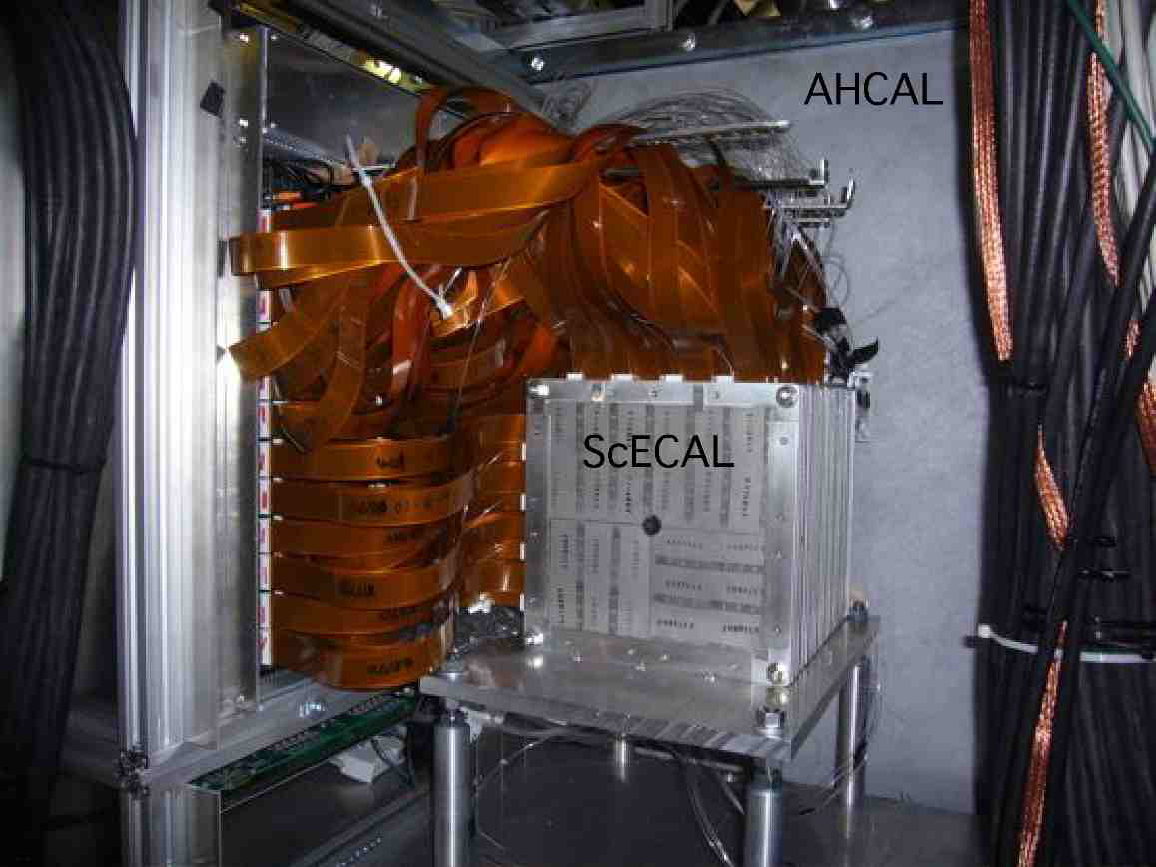
\includegraphics[width=1.\linewidth]{chap3/fig/photo_scecal2.pdf}
    \caption{} \label{fig:ScECALPhysics}
  \end{subfigure}
  \hfill
  \begin{subfigure}[t]{0.49\textwidth}
    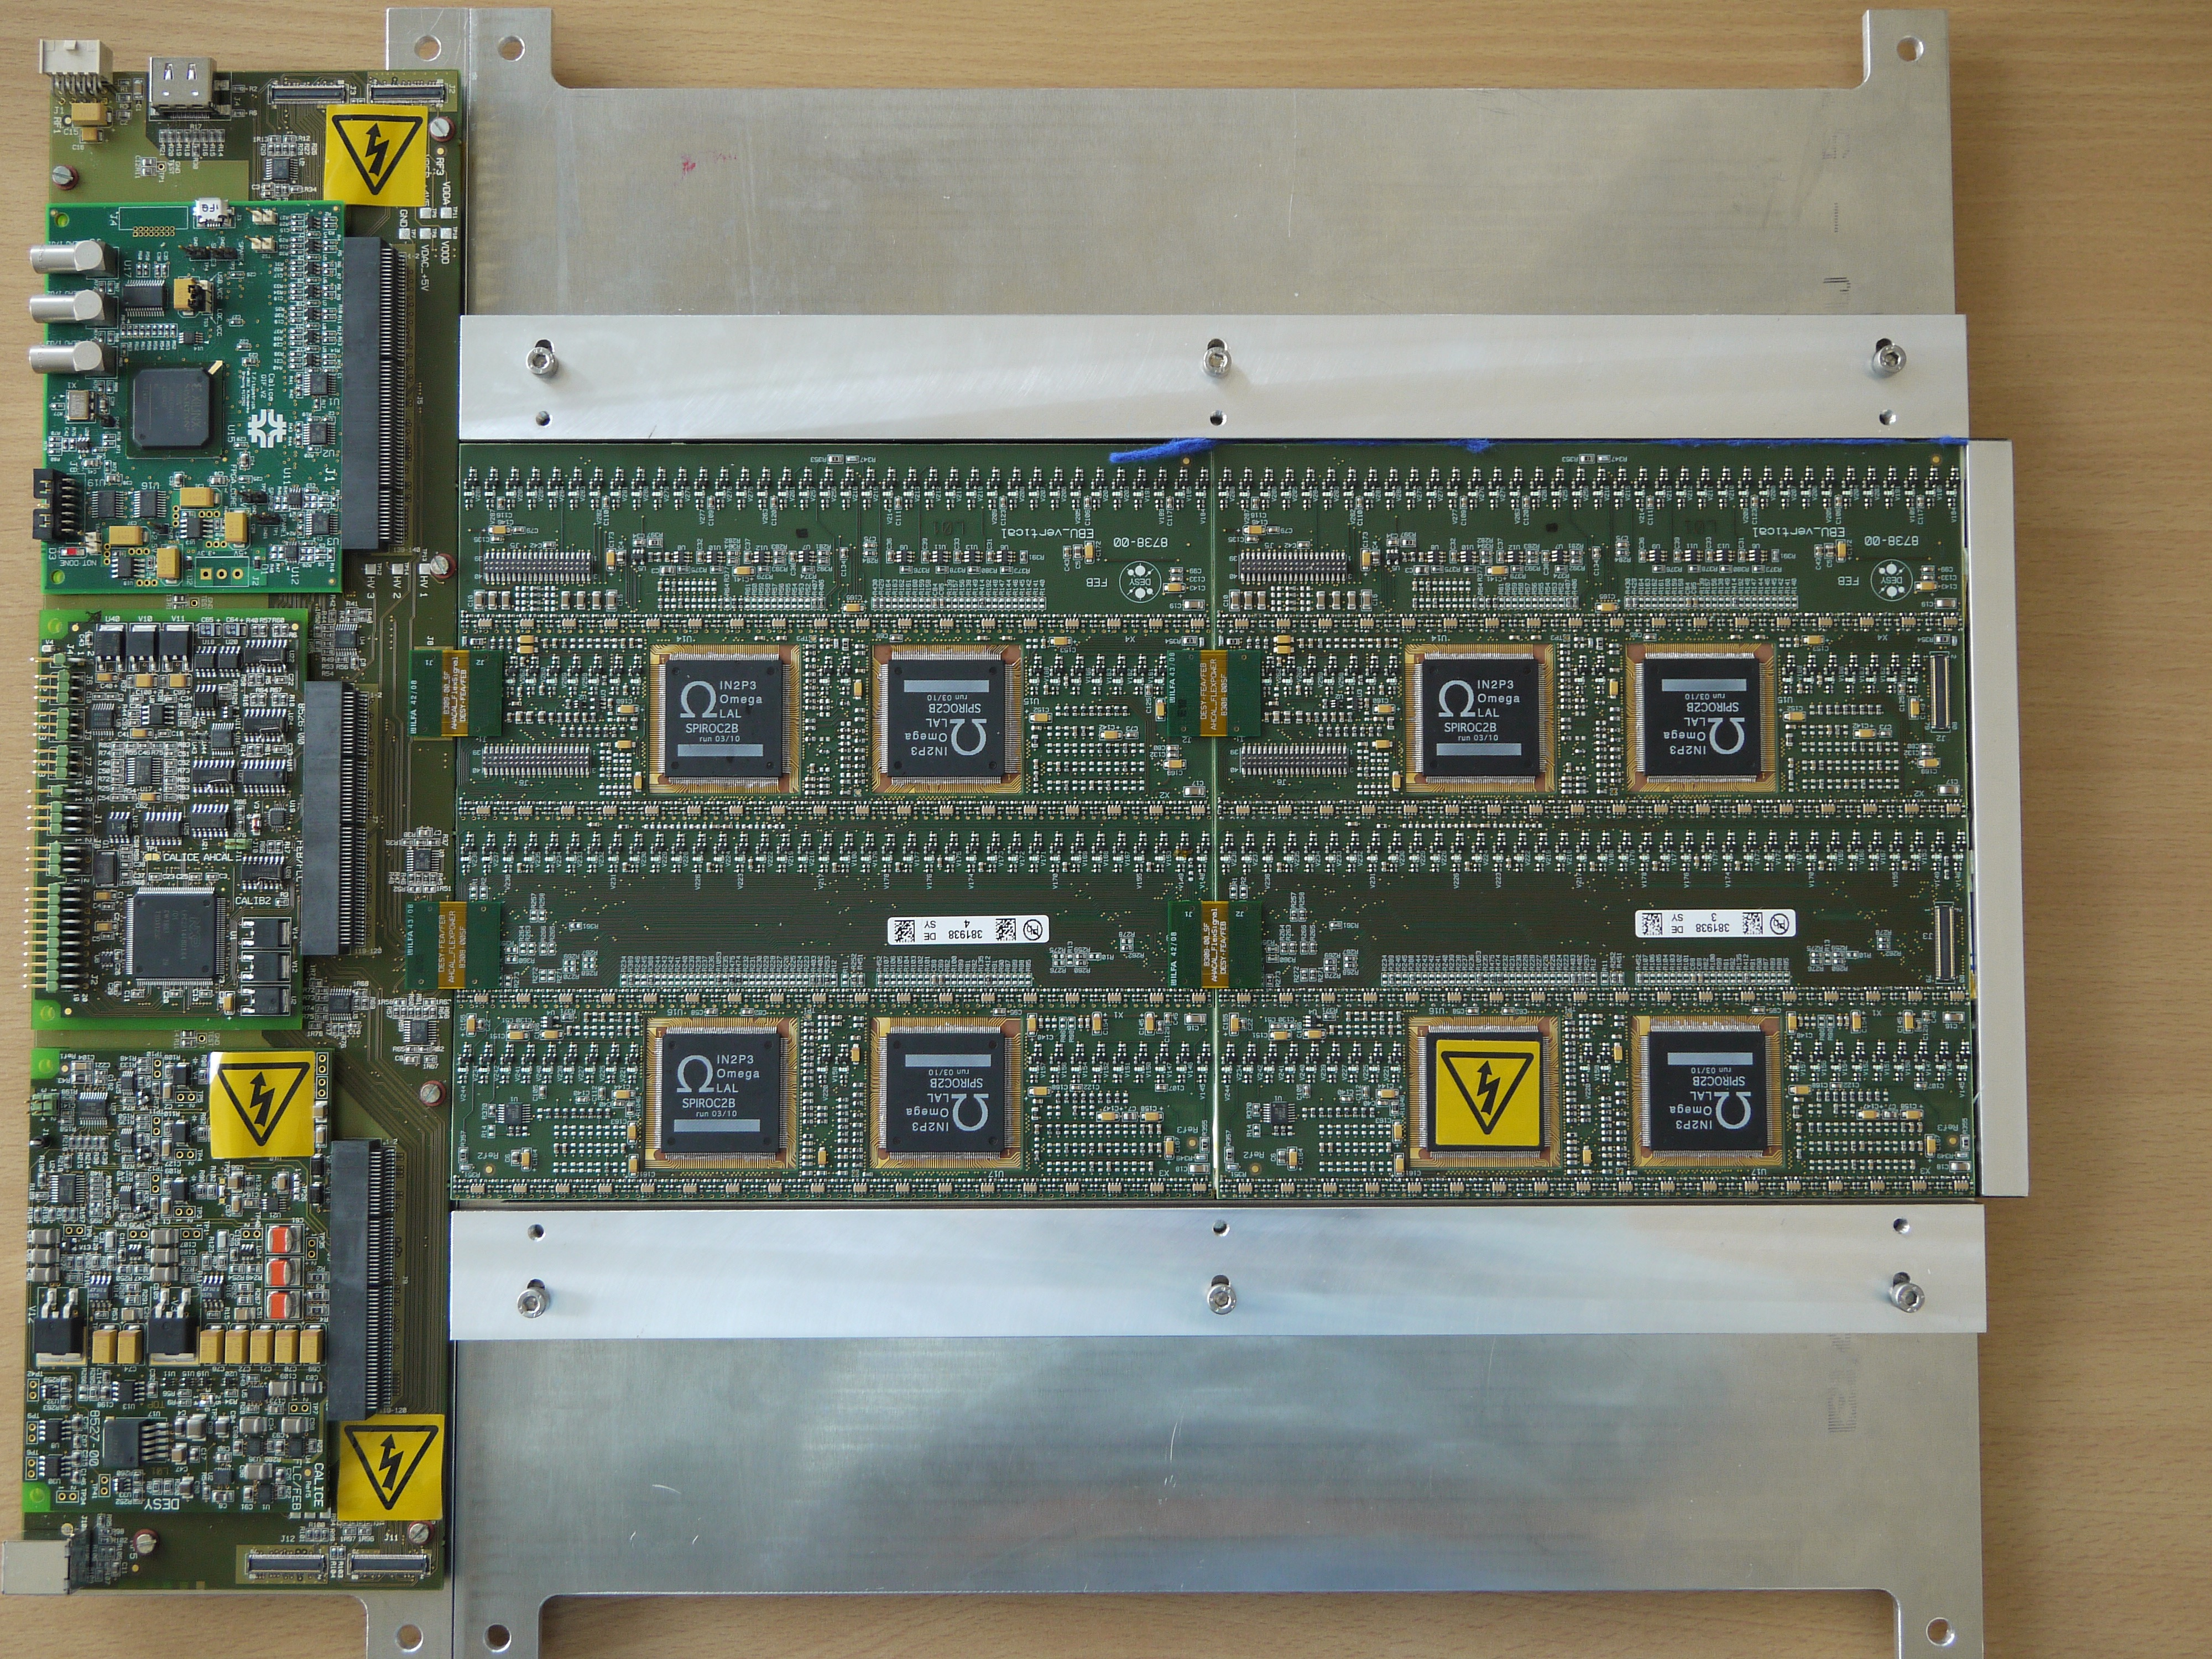
\includegraphics[width=1.\linewidth]{chap3/fig/P1060076.jpeg}
    \caption{} \label{fig:ScECALTechno}
  \end{subfigure}
  \caption{\subref{fig:ScECALPhysics}) Photo of the ScECAL physics prototype with the Fe-AHCAL at FNAL. \subref{fig:ScECALTechno}) Photo of the top side of the technological ScECAL prototype.}
\end{figure}

To look forward, a technological prototype is now developed to accommodate the front-end electronics into the layer to reduce the amount of dead material due to cabling. An ECAL Base Unit (EBU) has 144 scintillator strips of dimensions 45$\times$5$\times$2 mm$^3$. Each EBU has a transverse dimension of 180$\times$180 mm$^2$. The design of the EBU is derived from the HBU design (see section \ref{sec:AHCAL}).

The strips don't have a WLS fiber due to improvements in SiPM technology for the detection of blue light ($\sim$ 450 nm). Several designs in SiPM and scintillator strip shape are being studied to optimize light collection. Moreover by using a strip splitting algorithm (SSA) \cite{Kotera:2014psa}, an effective granularity of $5\times5$ mm$^2$ can be achieved.

In this thesis (see section \ref{sec:TBsetup}), two designs were used in testbeam at CERN, a bottom-side readout and baseline readout design. The former uses 10k pixels surface-mounted SiPM, the latter uses 1.6k pixels SiPM placed on the side of the strips. Each SiPM are read out by an ASIC, the \acrshort{spiroc2b} (see section \ref{sec:SPIROC2B}). Each layer is equipped with four SPIROC ASICs. Each channel has also an integrated LED calibration system in order to monitor the SiPM gain.

\section{Hadronic Calorimeters}
\label{sec:HadCal}

The CALICE collaboration is developing several hadron calorimeters concepts. Each concepts are varying in the granularity from $3\times3$ cm$^2$ to $1\times1$ cm$^2$ but as well in the precision of the amplitude information. The Digital HCAL and Semi-Digital HCAL calorimeter concepts are using digital information of the amplitude by counting the number of hits on 1 bit or 2 bits. The AHCAL calorimeter concept relies on the full analog information of the amplitude. A detailed comparison study of these different calorimeter concepts has been done and can be seen in \cite{Neubueser2016}.

\subsection{Digital HCAL}

The Digital Hadron Calorimeter (DHCAL) prototype \cite{Bilki:2013bea} is a sampling calorimeter based on Resistive Plate Chambers (RPCs) \cite{BEDJIDIAN2010120} gaseous technology. The DHCAL uses a 1-bit readout system based on the assumption that the deposited energy of a particle is proportional to the number of hits over a given threshold as a first order.

The DHCAL consists of 38 active layers of an active area of $1\times1$ m$^2$. The chambers are in a cassette with a front copper plate 2 mm thick and back steel plate 2 mm thick. They are inserted into the same steel absorber structure used of the AHCAL into gaps 1.4 cm wide. A schematic of the cross-section of a DHCAL layer is shown in figure \ref{fig:DHCALCross}.

The readout anode of the RPC is segmented into $1\times1$ cm$^2$ pads, read out by 2 front-end boards for each RPC (for a total of 6 boards for a layer) hosting 24 chips each for a total of 144 chips per layer. Each chip reads out 64 pads. The prototype accounts for a total of 350 208 channels.

\begin{figure}[htbp!]
  \centering
  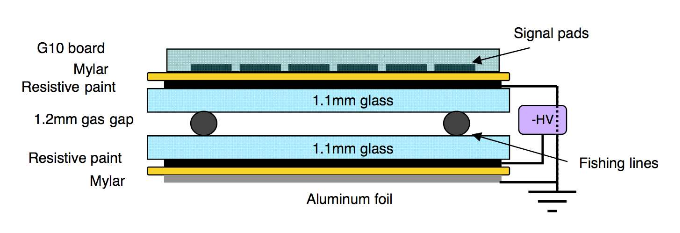
\includegraphics[width=0.9\linewidth]{chap3/fig/Cross-section-DHCAL.png}
  \caption{Cross-section of an active RPC layer in the DHCAL prototype. Taken from \cite{1748-0221-3-05-P05001}.} \label{fig:DHCALCross}
\end{figure}

This prototype has been used in the testbeam facilities at CERN and Fermilab. A preliminary analysis of testbeam data shows that an energy resolution of $\frac{35.1\%}{\sqrt{E}}$ stochastic and 12.4\% constant term has been achieved in a positron beam. More details about the DHCAL prototype can be seen in \cite{Neubueser2016}. However, this can be improved to around $\frac{13\%}{\sqrt{E}}$ stochastic and 6.2\% constant term with the DHCAL with minimum absorbers (Min-DHCAL) \cite{Freund:2016wvz}.

\subsection{Semi-Digital HCAL}

The Semi-Digital Hadron Calorimeter (SDHCAL) prototype \cite{1748-0221-10-10-P10039} uses also RPCs technology for particle detection. The SDHCAL consists of 48 active layers. Each active layer consists of RPCs with a gap of 1.2 mm filled with gas and a readout electrode segmented in $1\times1$ cm$^2$ pads.

The active layers are inserted into a steel absorber structure of 1.5 cm thick plates. In total, the SDHCAL prototype features 442 368 channels. More detail about the SDHCAL can be found in \cite{1748-0221-10-10-P10039}.

\begin{figure}[htbp!]
  \centering
  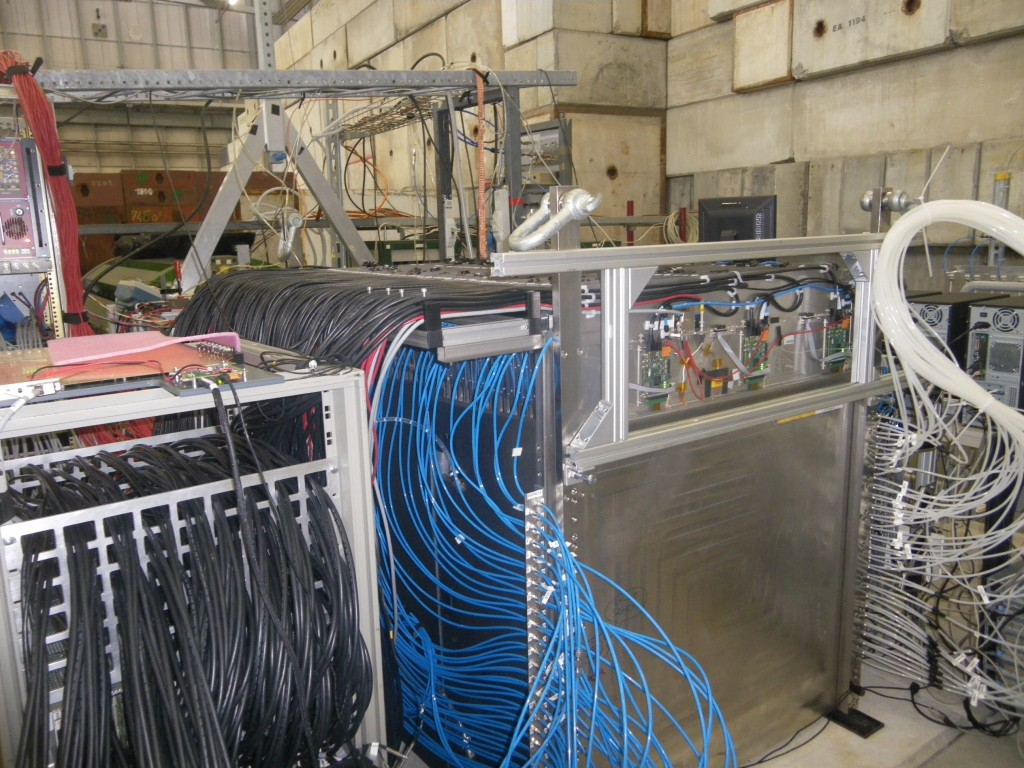
\includegraphics[width=0.7\linewidth]{chap3/fig/SDHCAL.jpg}
  \caption{Photo of SDHCAL at CERN in 2012.} \label{fig:SDHCAL}
\end{figure}

The readout is performed by the HARDROC ASIC \cite{HARDROC:IEEE} which can readout up to 64 channels. Instead of using 1-bit readout scheme like the DHCAL, the SDHCAL uses a 3-bit readout system corresponding to three coarse thresholds.

The SDHCAL does not provide direct timing measurement. A timestamp with a precision of 200 ns corresponding to the internal clock of the ASIC can be applied to hits.

The SDHCAL has been tested in various beam types at the CERN SPS facility in 2012. A picture of the prototype is shown in figure \ref{fig:SDHCAL}. The first results shows an energy resolution that goes from 14.9\% at 30 GeV to 9.5\% at 80 GeV with pion beams \cite{Buridon:2016ill}.

\subsection{Analog HCAL}
\label{sec:AHCAL}

The Analog Hadronic calorimeter uses scintillator-based tiles readout by Silicon Photomultipliers. Before discussing about the prototype, a short introduction about Silicon photomultipliers and the readout electronics is presented.

\subsubsection{Silicon Photomultipliers}
\label{sec:SiPM}

Semi-conductors detectors have been used since more than 50 years and are still a major research topic in high energy physics \cite{1748-0221-4-04-P04004, Garutti:2011qv, Garutti:2017ipx}. \textit{Silicon photomultipliers} (\acrshort{sipm}) are semi-conductors used to measure light amplitudes down to the single photon. SiPMs are composed of an array of \textit{Avalanche Photodiodes} (\acrshort{apd}) pixels operated in Geiger-mode. The pixels are all connected in parallel to a common cathode and anode. Nowadays, thousands of pixels can be integrated into a few $mm^2$ area. A picture of a surface-mounted SiPM is shown in figure \ref{fig:SMD_SiPM}.

\begin{figure}[htbp!]
  \centering
  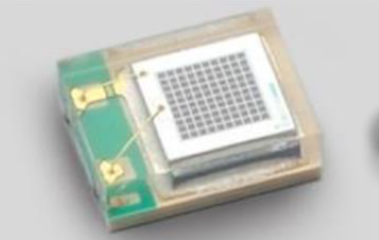
\includegraphics[width=0.4\linewidth]{chap3/fig/SMD_SiPM.png}
  \caption{Picture of a surface-mounted SiPM. The picture shows the SiPM package as well the grid of pixels.} \label{fig:SMD_SiPM}
\end{figure}

Each pixel is operated in reverse bias ($V_{bias}$), in the order of 30-60 V, larger than the \textit{breakdown voltage} ($V_{bd}$). When a photon is absorbed, an electron-hole pair is created in the depletion region by the photo-electric effect. This electron is accelerated by the electric field and starts to create a self-sustained avalanche or \textit{Geiger discharge} by impact ionization, rendering the diode conductive. A serial \textit{quenching resistor} ($R_q$) reduces the effective voltage of the pixel below $V_{bd}$ thus quenching the avalanche. Each pixel deliver a charge $Q$ such as
\begin{equation}
  Q = C_{px} \times (V_{bias} - V_{bd})
\end{equation}
where $C_{px}$ is the capacitance of the pixel which is typically around few pF and depends on the geometry and doping profile of the pixel. $V_{bias} - V_{bd}$ is the over-voltage or excess voltage over the breakdown voltage.

Following this equation, $Q$ characterizes the gain of the SiPM and is proportional to the over-voltage. $V_{bd}$ is temperature dependent, effectively increasing with the temperature. Thus the SiPM gain show an anti-correlation as a function of the temperature in the range of -1\%/K. Similarly, the \textit{quantum efficiency or photon detection efficiency} (\acrshort{pde}), the probability to initiate a Geiger discharge, has an inverse correlation with temperature and increases with $V_{bias} - V_{bd}$.

Once an avalanche has stopped, the effective voltage of the pixel can return to $V_{bias}$ with the \textit{recovery time} $R_q \cdot C_{px}$ in the order of hundred nanoseconds before the pixel can fire again. Carriers trapped in defects in the silicon matrix introduce new levels of energy in the conduction band, a release of these carriers causes \textit{afterpulsing} in a period of 50-100 ns after firing.

The measured total charge is the sum of all the fired pixels. With a good uniformity in pixel capacitance and low-noise electronic amplification, the SiPM gain can be measured in-situ by illuminating the SiPM with short and low amplitude light pulses giving a \textit{single-photon spectra} (SPS) as shown in subsection \ref{subsec:GainCharac}.

Due to the finite number of pixels and the recovery time of the pixels in the order of several nanoseconds, the response of a SiPM is non-linear and can be at a first order parametrized as
\begin{equation}
  N_{fired} \approx N_{total} \times (1 - e^{\frac{- N_{\gamma} \cdot PDE}{N_{total}}})
\end{equation}
where $N_{total}$ is the total number of pixels, $N_{\gamma}$ is the number of incoming photons and $PDE$ is the photon detection efficiency. This parametrization can describe the data very well at low light levels but can significantly differ with a high number of photons \cite{Kotera:2015rha}.

An avalanche can be initiated by a photon but also free carriers in the depleted layer. The rate of the latter \textit{dark noise} increases with $V_{bias} - V_{bd}$ and the temperature. A dark rate of 100 kHz to several MHz per mm$^2$ is produced by typical SiPMs. This dark count rate falls dramatically when increasing the threshold of the readout electronics and typically the increase of the threshold by 1 photo-electron amplitude reduces the dark rate by around one order of magnitude.

Geiger avalanches in a pixel can produce photons that can travel to the nearest pixel and trigger an avalanche. This is referred as \textit{optical cross-talk}. This effect is in the order of 3-10\% for typical SiPMs and can be mitigated by reducing the operating voltage, adding an optical absorber or trenches between pixels.

In the last decade, significant improvements in the manufacturing of SiPMs have been achieved and they are commercially available. The PDE range has been improved to be sensitive down to near ultraviolet light (300-400 nm) up to infrared light (800-1000 nm). The dark noise rates have been reduced as low as few tens of kHz at room temperature. The introduction of trenches between pixels in the substrate have enabled to reduce the cross-talk probability under 1\% \cite{Liu:2015cpe}. The uniformity improvements within one production batch reduce the need for individual bias adjustment. And finally, SiPMs with a very high number of pixels ($\geq$10000) are available, improving the range of linear response and increase the dynamic range but at the detriment of noise rates and PDE.

For the Analog Hadronic Calorimeter, a specific chip, the SPIROC2B has been developed to readout Silicon photomultipliers integrating all the requirements for the ILD detector. The next section will present the chip in details.

\subsubsection{The SPIROC ASIC}
\label{sec:SPIROC2B}

The SPIROC (SiPM Integrated Read-Out Chip) \cite{5401891} is a dedicated ASIC to readout and digitize the signal of SiPMs. The ASIC needs to satisfy the AHCAL requirements that are:

\begin{itemize}
  \item Readout and digitization of the SiPM signal.
  \item Small footprint for integration into the active layers between absorbers.
  \item Has a low power consumption under 25 mW per channel to avoid the need for active cooling.
  \item Operates in the power-pulsing scheme to reduce the power consumption and send the data between bunch-trains.
  \item Provides individual channel gain and bias voltage adjustment.
  \item Provides auto-triggering with adjustable threshold to reduce the data volume.
  \item Provides timing information of the SiPM signal
\end{itemize}

The SPIROC ASIC is developed by the OMEGA group \cite{OmegaWeb} to fulfill the AHCAL requirements. The SPIROC provides the readout for 36 SiPM channels capable to measure the charge and time for each channel. Each channel is equipped with a capacitor-array, called memory-cells, with a depth of 16 events to store the charge and time measurement. A 12-bit Wilkinson ADC is used to digitize the charge and time measurement stored in the capacitor array. The digitized signal is then stored into a RAM buffer.

Each channel can be tuned in bias voltage with a 8-bit Digital to Analog Converter (\acrshort{dac}) corresponding to a voltage range between -4.5V and 0V. Each channel, has a configurable low-noise charge pre-amplifier gain (between 100 fF to 1500 fF) operating in high gain (HG) or low gain (LG) to cover a high dynamic range between 1 to several thousand photoelectrons.

The time measurement is digitized using a 12-bit Time to Digital Converter (TDC). The TDC is a voltage ramp with a designed resolution of 100 ps if operated in ILC-like conditions (ramp length of 200 \si{\nano\second}). In testbeam, the theoretical time resolution is around 1.9 ns (ramp length of 4 \si{\micro\second}).

\begin{figure}[htbp!]
  \centering
  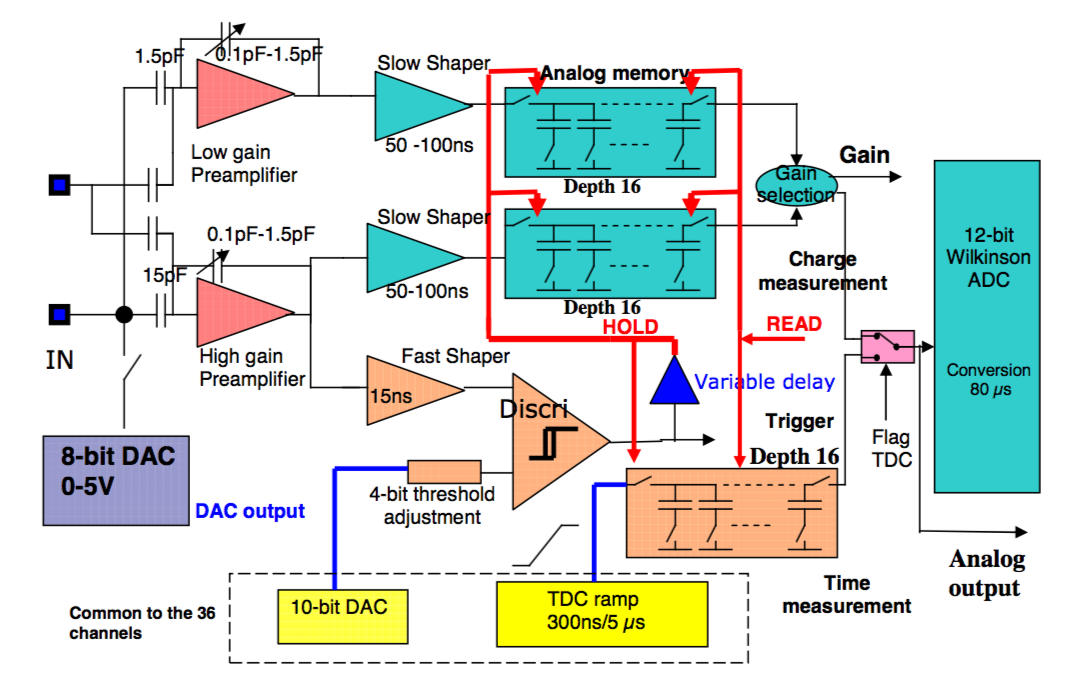
\includegraphics[width=0.7\linewidth]{chap3/fig/SPIROC2B_schematic.png}
  \caption{Schematic of the analog signal path of the SPIROC2 for a single channel \cite{SPIROC2_datasheet}.} \label{fig:SPIROC2B_sche}
\end{figure}

The chip can be operated in either external trigger mode (ET) or auto-trigger mode (AT). In external trigger, the signal of each cell is sampled synchronously to an external signal. This mode is used to measure the SiPM gain using the integrated LED system of the AHCAL which is described in section \ref{subsec:GainCharac}. The auto-trigger capabilities of the SPIROC are provided by a fast shaper and a discriminator. The threshold of the discriminator is configurable with a 10-bits DAC and is common to the 36 channels. A 4-bit DAC provides channel-wise threshold adjustment. When a trigger happens, the signal of each cell is compared to a configurable threshold, if the signal is above the threshold, the signal is stored into one memory-cell. In addition, the ASIC provides the information of which channel triggered called a \textit{HitBit}. An external validation trigger can be provided to the ASIC to reduce SiPM noise. The time measurement is stored in another memory-cell when there is a trigger.

Once the 16 memory-cells are filled, no further hits can be stored. Hence, the memory-cells are read-out, digitized and the data is transferred out of the chip. The chip can be operated in power-pulsing mode where parts of the chips not needed in any given state of operation can be switched off. A schematic of the analog part of the SPIROC is shown in figure \ref{fig:SPIROC2B_sche}.

Several iterations of the chip have been made to fix bugs and improve the provided functionalities. In this thesis, the SPIROC2b has been used for a large AHCAL prototype used in testbeams at DESY and CERN. A new version, the SPIROC2e, is currently used for constructing a cubic meter AHCAL prototype.

\subsubsection{The AHCAL Prototype}

The Analog Hadron Calorimeter (AHCAL) is a sampling calorimeter using scintillator tiles as active material. The absorber structure can be either steel or tungsten. The AHCAL physics prototype \cite{1748-0221-5-05-P05004} consists of 38 active layers inserted in a steel structure of a cubic meter with 39 absorber plates 1$\times$1 m wide and 17.4 mm thick on average. The calorimeter has a total depth of 4.28 $\lambda_{\pi}$ (5.3 $\lambda_{n}$). The active layers consist of a steel cassette housing 216, for the 30 first layers, or 141, for the 8 last layers, scintillator tiles connected on a PCB as shown in figure \ref{fig:AHCALPhysics}. The tiles are 5 mm thick and have different sizes of 3$\times$3, 6$\times$6, 12$\times$12 cm$^2$. This accounts for a total of 7608 channels. The light produced in the scintillator is guided through a WLS fiber 1 mm thick that is inserted in the tile to a SiPM. The SiPM sensitive area is 1.1$\times$1.1 mm$^2$ containing 1156 pixels which were produced by the MEPhi/PULSAR group in Russia.

The performance of this prototype has been demonstrated in several beam types. For electrons, the energy resolution of the AHCAL measured is $\frac{21.7\%}{\sqrt{E}}$ stochastic and <1\% constant term \cite{CAN034}. For pions, the intrinsic energy resolution of the AHCAL has been measured to be $\frac{57.6\%}{\sqrt{E}}$ stochastic and 1.6\% constant term. This can be improved to $\frac{45\%}{\sqrt{E}}$ stochastic term by using a technique called \textit{software compensation} \cite{SoftCompNew2012}. A picture of the prototype is shown in figure \ref{fig:AHCALPhysics2}.

\begin{figure}[htbp!]
  \centering
  \begin{subfigure}[t]{0.49\textwidth}
    \includegraphics[width=1.\linewidth]{chap3/fig/moduleinside.png}
    \caption{} \label{fig:AHCALPhysics}
  \end{subfigure}
  \hfill
  \begin{subfigure}[t]{0.49\textwidth}
    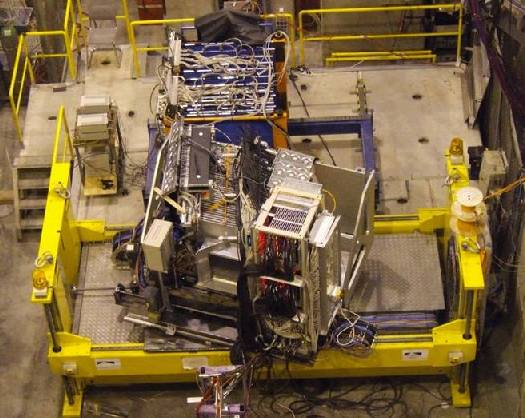
\includegraphics[width=1.\linewidth]{chap3/fig/CERN_setup.png}
    \caption{} \label{fig:AHCALPhysics2}
  \end{subfigure}
  \caption{\subref{fig:AHCALPhysics}) Photo of the active layer of the AHCAL physics prototype showing the layout of the differently sized tiles. \subref{fig:AHCALPhysics2}) Photo of the AHCAL physics prototype at CERN.}
\end{figure}

The AHCAL engineering prototype (EPT AHCAL) \cite{Felix:ProtoAHCAL} is currently being built. The goals of this prototype are to demonstrate the scalability of the AHCAL concept to a full linear collider detector. The HCAL Base Unit (HBU), see figure \ref{fig:AHCALHBU}, is 36 cm wide PCB holding 4 SPIROC2B ASICs for a total of 144 SiPM channels coupled to scintillator tiles of 30$\times$30$\times$3 mm size to be read out. Up to 6 HBUs can be connected together to form a \textit{slab}. A full AHCAL layer can be up to 3 slabs connected in parallel to a common set of readout (DIF), calibration (CALIB) and power modules (PWR). An integrated \acrshort{led} Calibration system \cite{KVASNICKA2012402} can deliver LED light pulses with amplitudes of a few photons up to saturation of the SiPM in order to calibrate and monitor each channel. Several designs of HBU and tiles have been produced to accommodate for soldering pin or surface-mounted (SMD) type SiPMs.

\begin{figure}[htbp!]
  \centering
  \begin{subfigure}[t]{0.37\textwidth}
    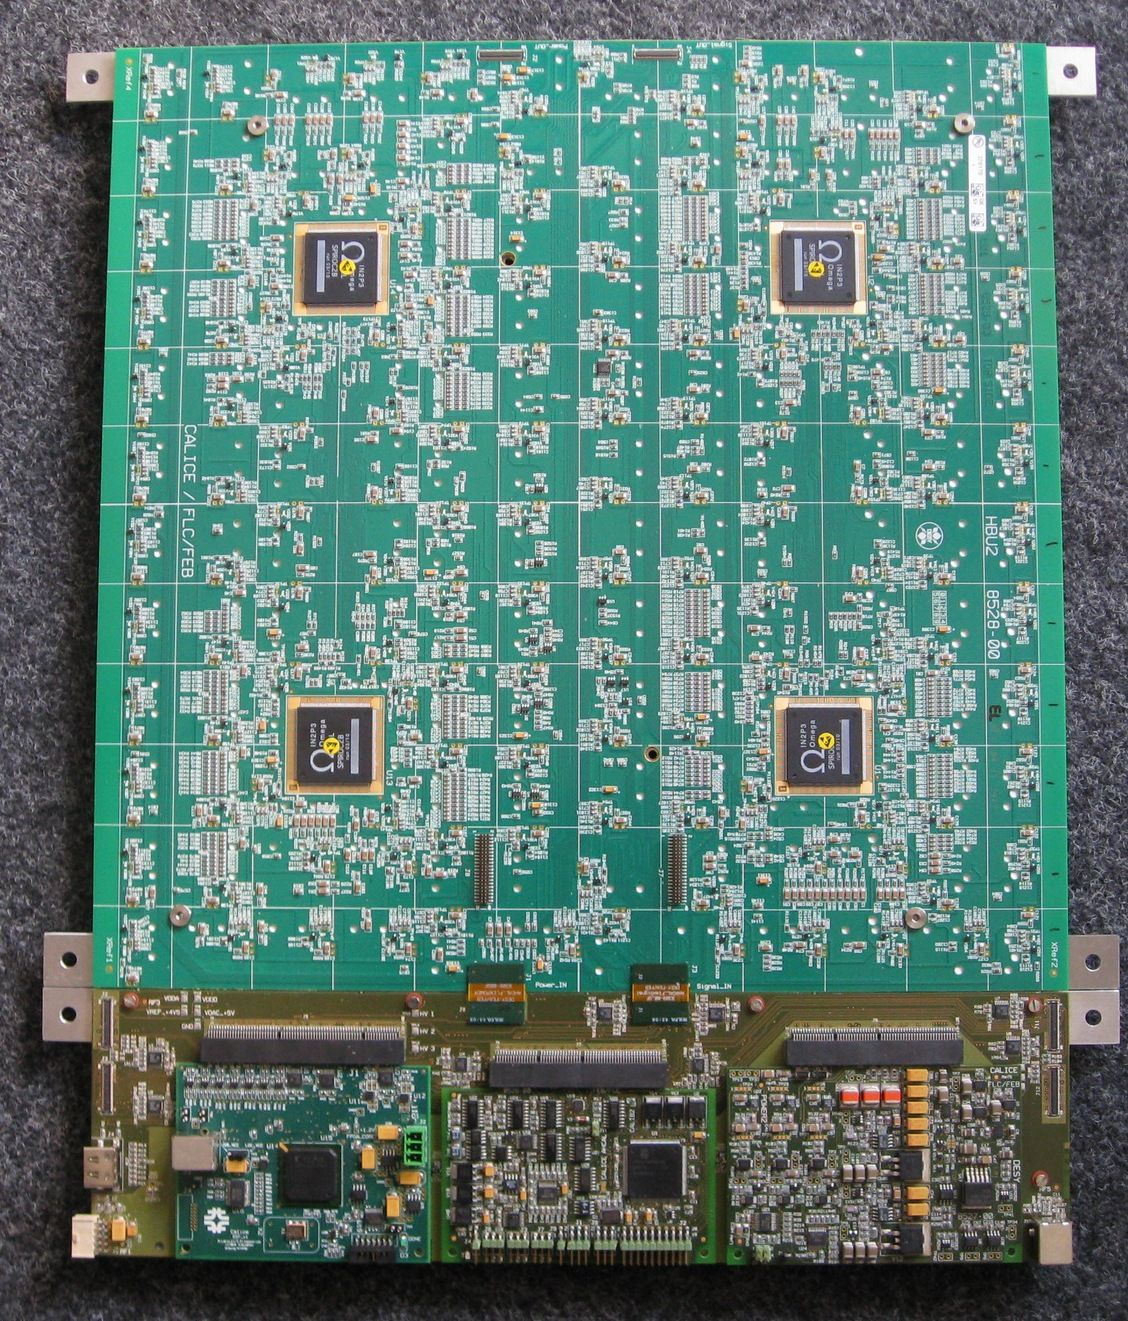
\includegraphics[width=1.\linewidth]{chap3/fig/CALICE_AHCAL_20120323.jpg}
    \caption{} \label{fig:AHCALHBU}
  \end{subfigure}
  \hfill
  \begin{subfigure}[t]{0.58\textwidth}
    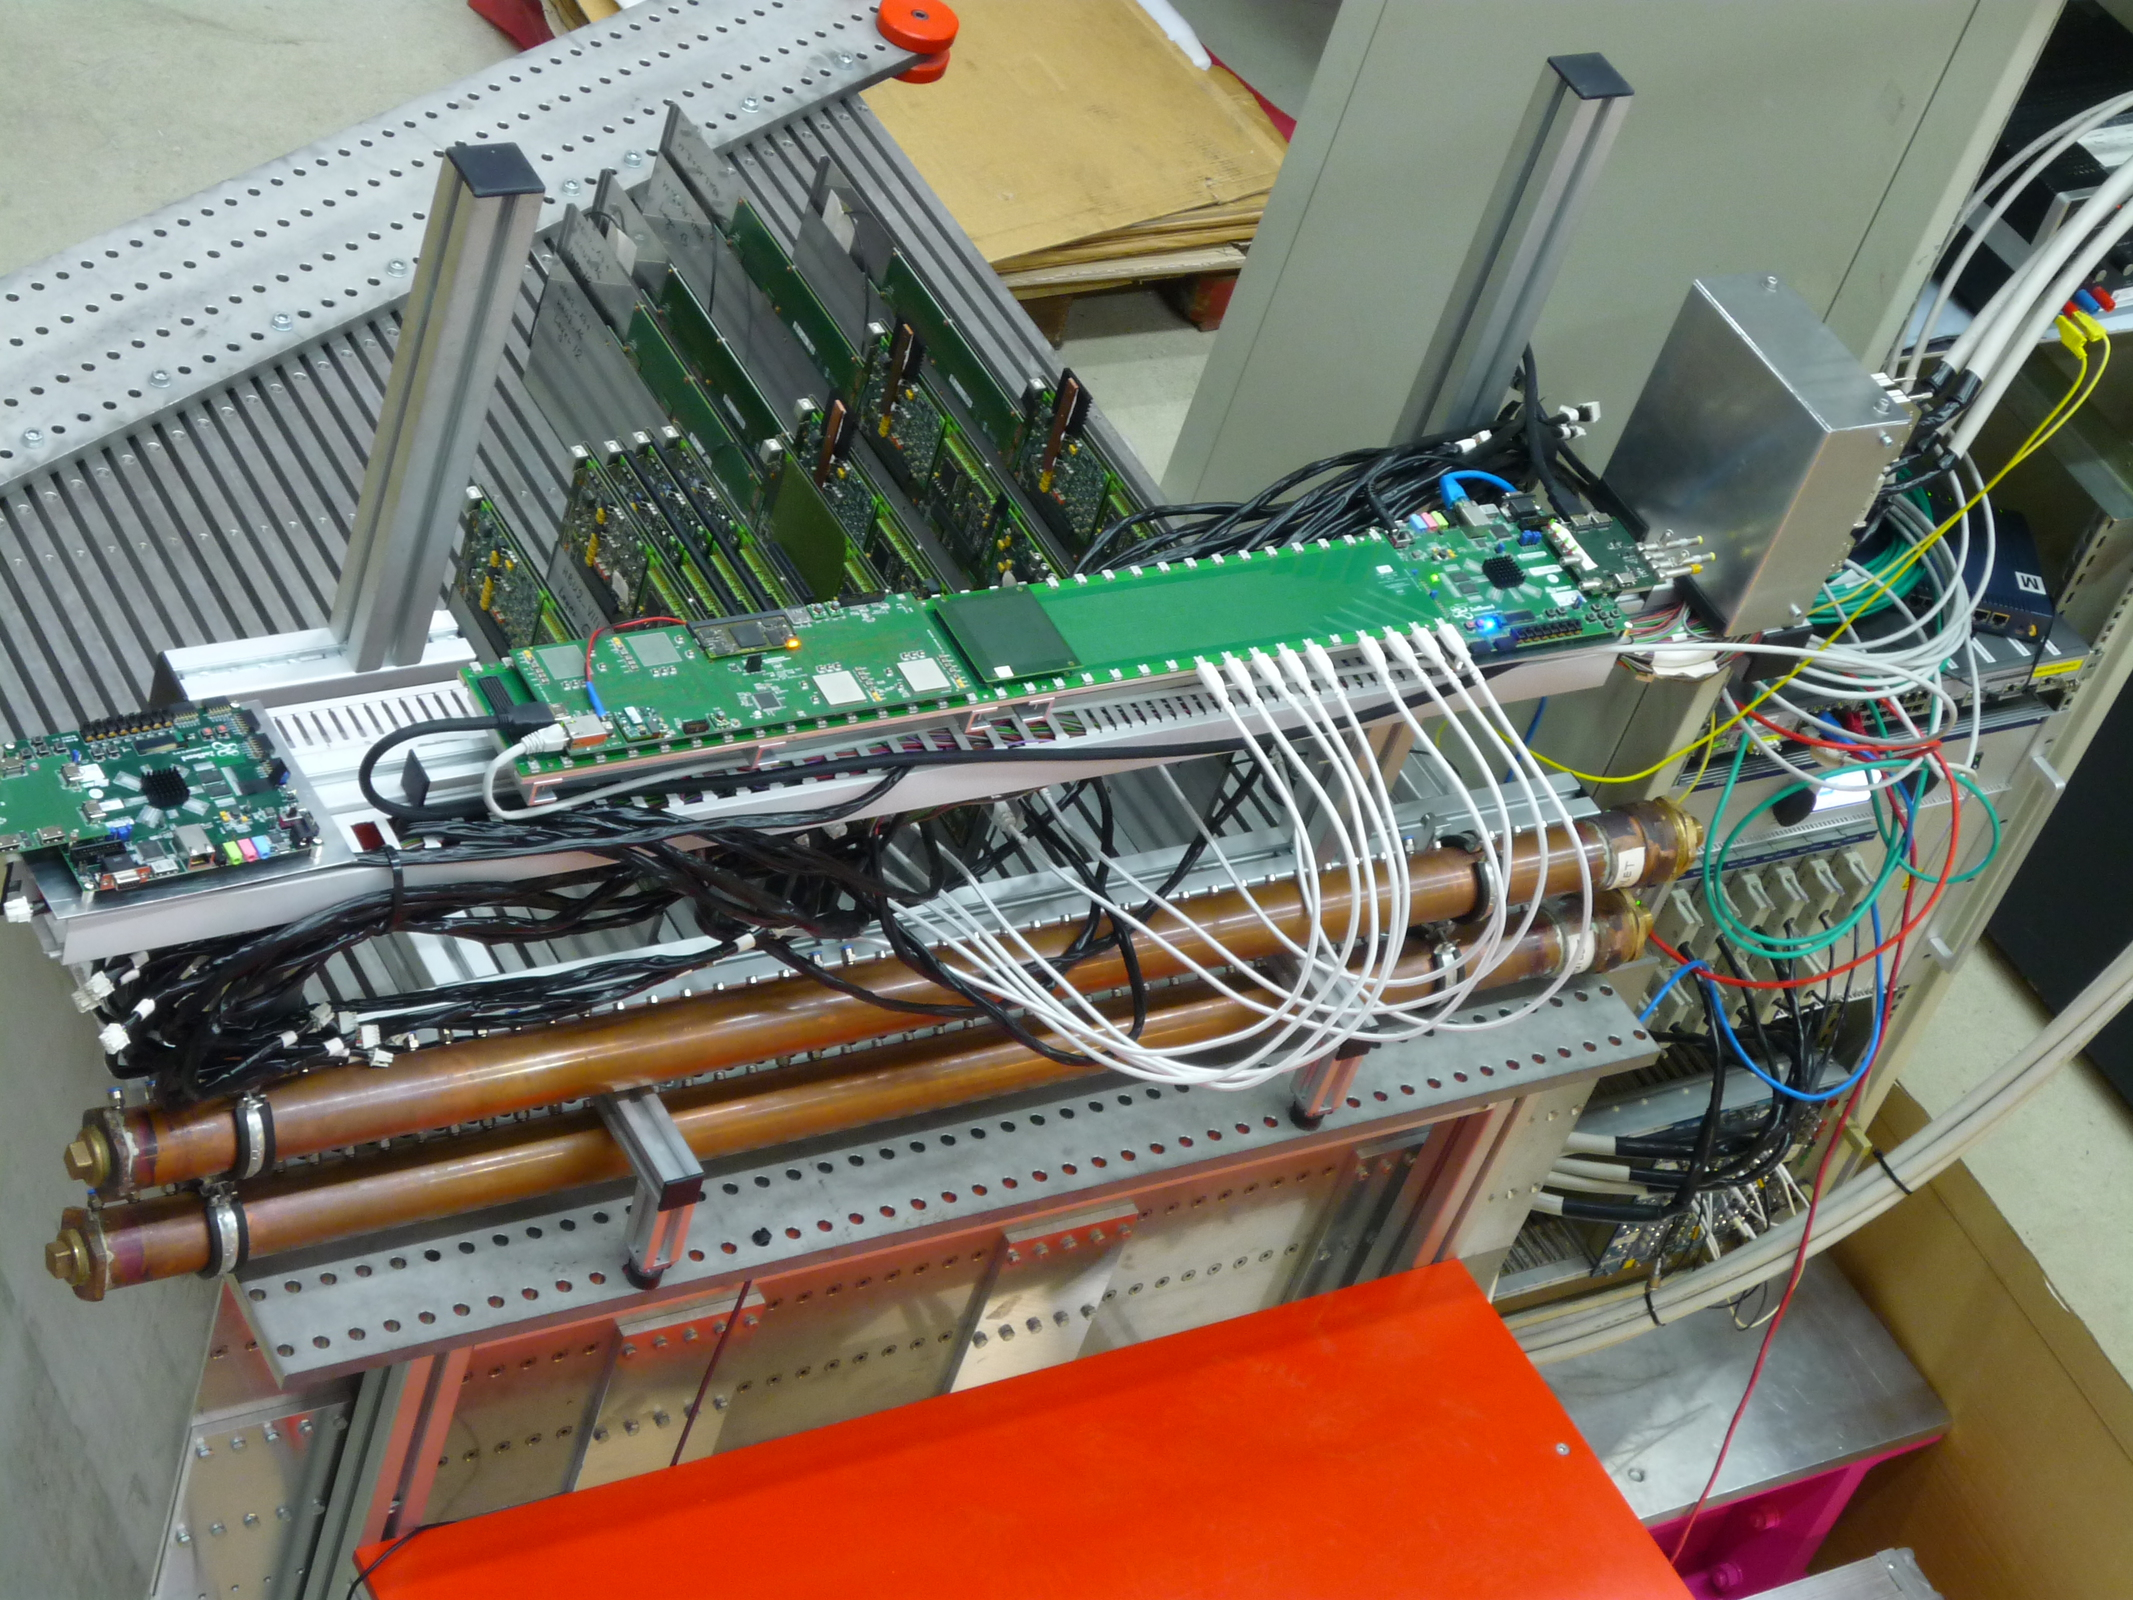
\includegraphics[width=1.\linewidth]{chap3/fig/P1030531_small.jpg}
    \caption{} \label{fig:AHCALStack2015}
  \end{subfigure}
  \caption{\subref{fig:AHCALHBU}) Top view of the HBU2 with SPIROC2b. \subref{fig:AHCALStack2015}) Picture of the AHCAL technological prototype in 2015 with several layers inserted.}
\end{figure}

A first step was achieved with the operation of 15 AHCAL layers in testbeam at the CERN SPS facility in July and August 2015. Various HBU designs with many types of SiPMs from different manufacturers have been used and served as a benchmark for the ongoing development of scintillator tiles concepts. The active layers were inserted into a steel absorber stack into gaps 9 mm wide with absorber plates that are 1.72 cm thick. The number of channel for this prototype accounts to a total of 3744. A picture of the steel stack with few inserted AHCAL layers is shown in figure \ref{fig:AHCALStack2015}. The data collected with this prototype is analyzed in this thesis (see from chapter \ref{chap:Commissioning} to \ref{chap:TimingPions}).

This prototype was composed of several different modules. The oldest ones were using a wavelength shifting fiber (WLS) that conducted the light on a SiPM whereas the newest modules were having wrapped tiles in a reflector foil without any WLS fiber inside due to the use of SiPMs that are blue light-sensitive. A picture of AHCAL tiles is shown in figure \ref{fig:TilesAHCAL2015}.

\begin{figure}[htbp!]
  \centering
  \begin{subfigure}[t]{0.43\textwidth}
    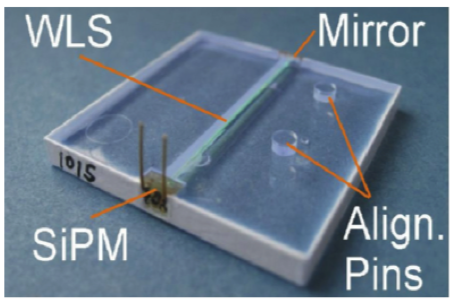
\includegraphics[width=1.\linewidth]{chap3/fig/AHCALTile_old.png}
    \caption{} \label{fig:AHCALTile_old}
  \end{subfigure}
  \hspace{2cm}
  \begin{subfigure}[t]{0.37\textwidth}
    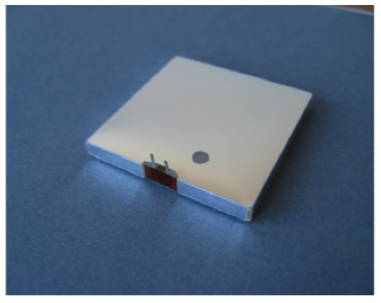
\includegraphics[width=1.\linewidth]{chap3/fig/AHCALTile_wrapped.png}
    \caption{} \label{fig:AHCALTile_new}
  \end{subfigure}
  \caption{The two different tiles used in the AHCAL technological prototype. The tile on the left is an older version with a WLS fiber and the tile on the right is a new design by University of Hamburg which is wrapped in reflective foil and has no WLS fiber.} \label{fig:TilesAHCAL2015}
\end{figure}

The current AHCAL DAQ system is fully capable of operating a full scale calorimeter prototype in testbeam in various configurations and is being extended to integrate with other DAQ systems of other detectors (CMS HGCAL prototype, Sc/SiECAL prototype...) and testbeam instrumentation (Telescope, Trigger Logic Unit (TLU)...) using the common EUDAQ framework \cite{Kvasnicka:CR_IEEE2016, Kvasnicka:2017bpx, Wing:2296332}.

\subsubsection{Current status of the AHCAL engineering prototype}

A first milestone has been achieved by the construction of the small prototype of 15 AHCAL layers in 2016. The goals for this prototype are:
\begin{itemize}
  \item The validation of the surface mounted tile-SiPM design using a Hamamatsu MPPC with 2700 px and the new HBU design.
  \item The evaluation of the performance of such calorimeter in electron beams at DESY.
  \item The operation of the detector in power-pulsing mode and in a magnetic field \cite{CR_IEEE2017}.
  \end{itemize}

In addition, this prototype has been used as backing calorimeter for the CMS HGCAL prototype for the HL-LHC upgrade \cite{Felix:AHCALMain2017_HGHCAL}.

\begin{figure}[htbp!]
  \centering
  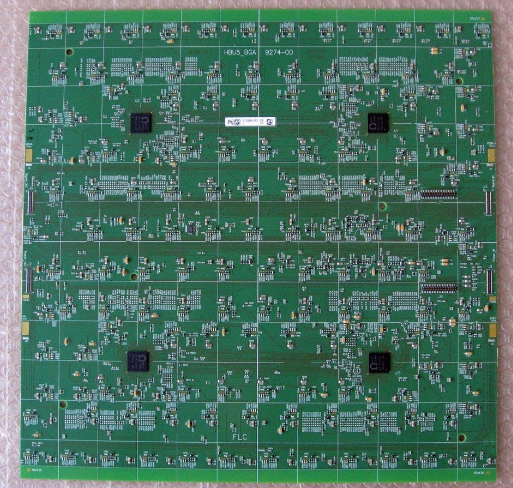
\includegraphics[width=0.45\linewidth]{chap3/fig/HBU5_BGA.png}
  \caption{Photo of the top view of the HBU5 with SPIROC2e used for the new AHCAL prototype.} \label{fig:HBU5_BGA}
\end{figure}

Concerning the assembly of HBU boards, for electric components, this is fully automatized. For the scintillator tiles, the assembly on a mass-production scale is being investigated and is currently being demonstrated for the production batch of HBU boards \cite{Phi:AHCALMain2017}.

The next milestone is the construction and operation of a full calorimeter prototype consisted of 40 $2\times2$ HBU layers equipped with the current surface-mounted MPPCs and tiles, in a steel absorber stack and using the SPIROC2e as front-end electronics, see figure \ref{fig:HBU5_BGA}. It is planned to be operated in power-pulsing mode in various electron and hadron beams at CERN in 2018 before the shutdown \cite{Felix:AHCALMain2017}.

\begin{center}
  \rule{0.5\textwidth}{.4pt}
\end{center}

In this chapter, the calorimeter concepts (electromagnetic and hadronic) of the CALICE Collaboration have been described. Concerning the hadronic calorimeters, 3 concepts have been presented. The DHCAL and SDHCAL use RPC gaseous technology to measure a signal on one or three bits readout scheme. The AHCAL uses scintillator-tiles coupled to a SiPM readout system to measure the analog signal of the deposited energy in each cell.

In this thesis, the data analyzed is compared to different simulations. Before discussing the analysis and the results, it is important to understand the differences between the simulation models. In the next chapter, the simulation and software tools relevant for this thesis are discussed.
